\section{Approach}
\label{sec:approach}

Given a natural language relation with its training relation
instances, our inference model first generates candidate 
schemas from its training relation instances, and then constructs a
probabilistic distribution over all the candidates.
Due to the lack of direct $\langle relation,\, schema \rangle$
training data, our learning model is distant supervised, we design
a data-driven function to label each candidate with ``silver'' 
score, and then perform the learning step based on ``silver'' labels.

% talk about model here
Suppose we have $N$ training relations in total.
We define $GEN(r)$ as the generation set of candidate schemas for 
the relation $r$.
The conditional probability of a schema $s \in GEN(r)$ is produced 
by log-linear model:
\begin{equation}
  p(s|r; \vec{w}) = 
    \frac { 
      exp \{ \vec{f} (s, r) \cdot \vec{w} \} 
    } { 
	  \sum\limits_{s' \in GEN(r)} { 
	    exp \{ \vec{f} (s', r) \cdot \vec{w} \} 
	  }
    },
\end{equation}

\noindent
where $\vec{f} (s, r)$ is the feature vector extracted from the
relation and the schema, and $\vec{w}$ represents the vector of
feature weights, which we are going to learn.
As mentioned above, we define the silver labeling function on a 
schema ranging from 0 to 1, which is denoted by $lb(s, r)$.
The silver labeling function approximates the correctness of one
schema, and the goal of training is to minimize the negative 
log-likelihood function of correct schemas over all the candidates.
The formal loss function is shown below:
\begin{equation}
J(\vec{w}) = \lambda \| \vec{w} \|_2^2 \! - \!  
  \frac {1} {N} \! 
  \sum\limits_{i=1}^{N} {
    log \! \sum\limits_{s \in GEN(r_i)} { 
	  lb(s, r) p(s|r; \vec{w}) 
	}
  },
\end{equation}

\noindent
where $\lambda$ is L2 regularization parameter.
In the following sections, we describe generation set, silver 
labeling function and feature functions in detail.


% then 3 step in detail
% 1. candidate generation (BFS + DFS)
\section{Candidate Schema Generation}
\label{sec:candgen}

We propose a search algorithm to collect 
candidate schemas from training relation instances.
The intuition is that we first find suitable skeletons 
as a starting point, and then recursively add constraints on 
previous schemas, producing more specific candidate schemas.

%7 sentences introducing bfs
%1. recap
%As outlined in \secref{sec:problem}, a skeleton is a path of KB 
%predicates which connects target variables $x_1$ and $x_2$.
%2. basic: bfs
For each relation instance $(e_1, e_2)$, 
we use breadth-first search from both ends 
to find all suitable skeletons that connect them in KB.
%3. problem of connection
%Due to various predicates and popular entities existed, a relation 
%instance could be linked through a large number of different skeletons.
%4. what's meaningless rep.
%Most of natural language relations are short phrases, a skeleton 
%with too many predicates is meaningless, and is less likely 
%to be a suitable representation.
%5. solution to filter
We limit the maximum number of edges of the skeletons to be $\tau$.
%6. why use minimal coverage
The number of input relation instances
covered by a schema $S$ is called the {\em support} of $S$, or
$sup(S)$.
To ensure the quality of the retrieved skeleton, we also
require that $sup(S) \ge \gamma$. 
%Also note that we always focus on well-descriptive skeletons, 
%rather than some occasional paths covering only a few entity pairs.
%7. say in detail
%In formal, we define another threshold $cov$ as the minimum 
%percentage of entity pairs among all positive instances covered 
%by a skeleton.
% Comment: we could describe the searching process in detail, like Matt's style "more formally, blabla..."


%18 sentences: bfs basic, search space limit, budget, diversity
%1. general speak
After candidate skeletons are produced, we deploy depth-first search on
each skeleton to obtain more specific schemas.
At each step of the search, we attempt to add an edge to any one node
on the skeleton. An edge can be added if the support of the 
new schema is larger than $\gamma$. 
This process continues recursively until
no new schemas can be found.
%3-6: basic limit on schema constraints
%3. why need limitation
%The searching space is a tree structure which grows exponentially,
%making the exhaustive searching intractable on a huge knowlege base.
%4. how to fix the search size
Each additionl edge on a variable node acts like a constraint on the variable.
In practice, multiple constraints on the same variable seldom make sense. 
Therefore, we require that at most one edge is added to any node 
on the skeleton.
%5. the intuition behind
%As mentioned before, natural language relations are always short
%phrases, which gives us the point that it's less likely to infer
%a comfortable structure for a relation with multiple restriction 
%imposed on a single element, and our restriction just follows 
%this intuition.
%6. the effect of limitation
Consequently, the maximal depth of the searching tree is $\tau+1$.

%7-11: budget base (why, budget+prune, criteria, how to prune, diversity)
%7. why need budget
Unfortunately, each node in a skeleton may be attached hundreds of
different predicate in a large KB. The overall search space, though
bounded by the constant depth, is still large.
%8. introduce budget+pruning
Inspired by beam search algorithm\cite{ney1992data}, we introduce a fixed size 
priority queue to store the set of candidate schemas for each relation.
Our goal is to fill this queue (an operational budget) 
with relatively higher quality
schemas. We simply use the support of each schema on the input instances
as the quality or priority of the schema. The idea is that a better schema
should cover more instances. Also since as we attach more edges to the schema,
the support monotonically decreases, we can use this 
monotonicity property to prune the search
space. At each step of the search, we enumerate all the possible new schemas
(with one new edge) and insert the best among them to the priority queue if the
queue is not full. If the queue is full, we compare the support of the 
schema to be inserted with the worst schema on the queue. 
If the current schema is better than the worst schema on the queue, 
the worst schema is replaced and
the search continued from the current best schema. 
Otherwise, we prune the search space and backtrack.

%while pruning strategies will be used to reduce 
%searching space so that poor candidates could be ignored.
%9. what's the criteria
%To this end, we use the number of instances covered by 
%a schema as the criteria to approximately measure its quality.
%%10. explanation of the criteria
%The reason is two-fold: we aim to keep those descriptive schemas in 
%the output candidates, since we output a bunch of schemas instead
%of only a few, we don't need a rather precise quality measurement,
%the idea that better schemas cover more positive instances is
%reasonable enough for our task; 
%and the size of coverages would never increase when the search goes
%deeper, which leads to a simple but effective pruning strategy.
%
%11-15. formal describe
%Now we explain the searching step in formal.
%% [A simple pseudo code is available]
%The beginning state of the searching is one skeleton, we enumerate
%all the constraints which are allowed to add on, each constraint 
%maps to a more specific schema.
%Then new schemas are ranked over their coverages by descending order,
%and we sequentially continue recursive searching on those schemas.
%When the searching state comes to a new schema $s_0$, we keep this 
%schema if there has enough room to keep candidates; 
%otherwise, we pick the schema $s_1$ which has the smallest 
%coverage among all kept schemas and compare their coverage.
%If $s_0$ has a larger coverage, then $s_1$ is discarded, we keep 
%$s_0$ and search deeper; otherwise, the current schema $s_0$ is 
%pruned, and we backtrace the searching process immediately.
%Finally, the output candidates are those schemas been kept when
%the searching is over.

%16-18. diversity
Finally, we would like the generated set of candidate schemas
to be diverse and not all similar to each other.
%The diversity of output schemas plays an important rule in the 
%learning parts.
%If most candidates are the same and only differ from one or two 
%constraints, we are actually wasting budgets because it contains
%much redundant information.
We thus maintain multiple priority queues, one for each skeleton.
The size of each queue is proportional to the support of the corresponding
skeleton.


% 2. silver labeling (ratio function)
\section{Silver Labeling Function}
\label{sec:label}

%18 sents.
%1. intro (2 sent)
With a schema $s$, a relation $r$ and its training instances as 
input, the silver labeling function $lb(s, r)$ approximately 
measures the correctness of the schema representing the relation.
The function follows a simple data-driven idea: a schema is more
confident to be correct, if it covers more positive relation 
instances and less negative instances. 
%2. incompleteness (3 sent)
A straightforword function can be derived by just calculate the 
proportion of instances covered in both positive and negative side.
However, the incompleteness fact of KB has not been taken into 
consideration: given a positive instance $\langle e_1, e_2 \rangle$,
where $e_1$ is a rare entity in KB, and its relationship with other
entities are not well connected, even a best schema (annotated by 
human) can't cover this entity pair, should this pair contributes
a negative evdience equally with those popular pairs not covered by
a schema?
The answer is no, so treating all positive and negative instances 
equally is not the best way to produce labeling function.

%3. group by e1 + formula (7 sent)
Now we introduce our solution to handle this problem.
The notations listed below are used in this secton:
\begin{itemize}
  \item $E_1(r)$: the set of distinct $e_1$ in training instances of $r$,
  \item $CV_s(e_1)$: all $e_2$ where $\langle e_1, e_2 \rangle$ is covered by $s$ in KB, 
  \item $PS_r(e_1)$: all $e_2$ where $\langle e_1, e_2 \rangle$ is in positive instances,
  \item $NS_r(e_1)$: all $e_2$ where $\langle e_1, e_2 \rangle$ is in negative instances,
  \item $PC_{sr}(e_1) = PS_r(e_1) \cap CV_s(e_1)$, and
  \item $NC_{sr}(e_1) = NS_r(e_1) \cap CV_s(e_1)$.
\end{itemize}

For positive part of training data, we define the confidence score 
of $e_1$ to the schema $s$ over relation $r$ as 
\eqnref{eqn:scp}:
\begin{equation}
\label{eqn:scp}
  sc_p(e_1, \! s, \! r) \! = \! \left\{
  	\begin{aligned}
	\! 1 / ( 1 \! + \! \ln \frac 
	  {\left| PS_r(e_1) \right|} 
	  {\left| PC_{sr}(e_1) \right|} 
	)    & ~ & PC_{sr}(e_1) \! \neq \! \varnothing  \\
	\! 0 & ~ & CV_s(e_1) \! = \! \varnothing        \\
	\! \frac {1} {
	  1 \! + \! \ln (\left| CV_s(e_1) \right| \! + \! 1)
	} \! - \! 1  & ~ & otherwise    \\
	\end{aligned}
  \right..
\end{equation}

These 3 branches in the formula represents different scenarios.
The first branch shows us that some positive $e_2$ are covered by 
the schema in KB, thus $e_1$ makes a confidence larger than 0:
The confidence reaches 1 if all positive instances are covered, 
and the scores decreases smoothly when more positive instance are
not covered by $s$.
The second branch encounters the problem of incompleteness: 
querying the shcema over $e_1$ returns nothing, without enough 
information, we can't make the statement that $s$ is not correct,
so we put a zero confidence here.
The last branch goes even worse: some $e_2$ are covered in the 
knowledge base, but neither is found in the positives instances.
Though KB incompleteness is still possible in this scenario, 
with more $e_2$ covered, the $e_1$ is more popular, which 
gives us a stronger evidence that $s$ is not correct.
Therefore, the confidence for the schema goes down from 0,
and become smaller when its coverage on $e_1$ goes larger, with
the minimum confidence as -1.

%4. negative side (3 sent)
Then we consider the negative part of training data.
Similar with \eqnref{eqn:scp}, negative relation instances also
provide confidence scores to the schema, 
defined in \eqnref{eqn:scn}:
\begin{equation}
\label{eqn:scn}
  sc_n(e_1, \! s, \! r) \! = \! \left\{
    \begin{aligned}
	\! -1 / ( 1 \! + \! ln \frac
	  {\left| NS_r(e_1) \right|}
	  {\left| NC_{sr}(e_1) \right|}
	)            & ~ & NC_{sr}(e_1) \! \neq \! \varnothing  \\
	\! 0         & ~ & CV_s(e_1) \! = \! \varnothing        \\
	\! 1 \! - \! \frac {1} {
	  1 \! + \! ln (\left| CV_s(e_1) \right| \! + \! 1)
	}            & ~ & otherwise \\
	\end{aligned}
  \right.,
\end{equation}

\noindent
where the first scenario makes the confidence score smaller than 0
(negative instances are covered by $s$); again the second scenario
faces the problem of KB incompleteness and we can't decide the 
quality of schema by this $e_1$; the last scenario shows us a
confidence score larger than 0, since all entity pairs it covered 
on $e_1$ are not negative, and the score increases monotonically 
when the size of coverage increases.

%5. summary  (3 sent)
In summary, each distinct $e_1$ from the training data of $r$ gives
us confidence scores on the side of both positive and negative
instances, ranging from -1 to 1.
Our silver labeling function takes all the confidences and 
averages them into the score from 0 to 1:
\begin{equation}
\begin{aligned}
  lb(s, & r) = 
  \frac {1} {2 \cdot \left| E_1(r) \right|}
  \sum\limits_{e_1 \in E_1(r)} \{ 
    1 + \\
	& \alpha \cdot sc_p(e_1, s, r) 
	+ (1 - \alpha) \cdot sc_n(e_1, s, r)
  \},  \\
\end{aligned}
\end{equation}

\noindent
where $\alpha$ controls the tradeoff between positive and negative
instances.


% 3. learning step (feature selection)
\subsection{Feature Engineering}
\label{sec:feature}
Our system makes use of three types of features: local geo-spatial
features, global geo-spatial features and non-geo-spatial features.
Each feature is calculated and assigned to every individual road segment
on the road map. Next we explain these features in more details.

\subsubsection{Local Geospatial Features}
The main intuition behind local geospatial features is that the traffic 
condition may depend on the the density of the local road network and also
the type of POIs near by. If there are too many traffic lights in a short stretch
of road, chances are the traffic will be slow. On the other hand, if there is a
school by the road, traffic will be affected in the morning and afternoon due to
the delivery and pick up of school childrens by their family. 

To measure the density of the road network, 
we calculate the average distance between two adjacent traffic lights \footnote{This is calculated by averaging from three pairs of consecutive crossroads
starting from the road segment in question.} in
both directions of the road segment under examination.
We divide all POIs on Baidu map into 37 types.
This classification is obtained by merging some of the finer categories which
were defined by Baidu's 2-level POI type hierarchy. Our second type of local 
features are the distribution of these 37 types of POI in the vicinity of the
target road segment, computed in both directions of travel 
(see \figref{fig:poifeature}). 

\begin{figure}[th]
	\centering
	\resizebox{\columnwidth}{!}{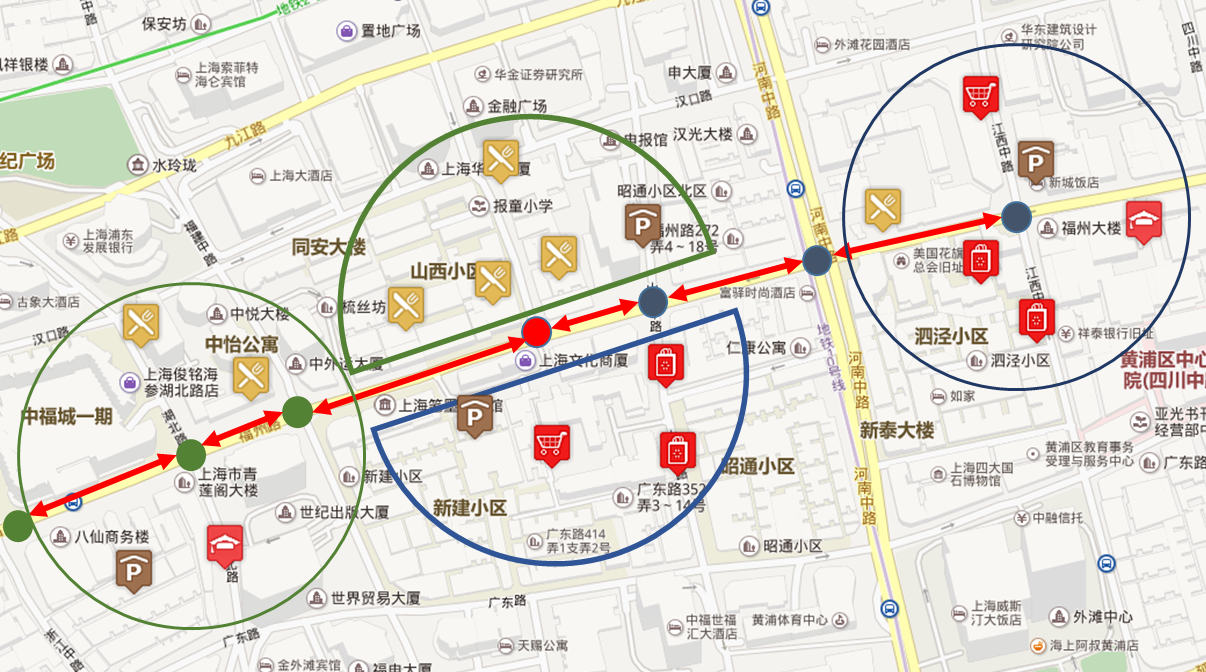
\includegraphics{figures/features/poi.png}}
	\caption{Local Geospatial Features}
	\label{fig:poifeature}
\end{figure}



%While digging on the information we have and brainstorming to achieve a list of features that may become useful, the first set of features that comes into our mind is the information that could best describe the local situation of a given place or point. For example, the road network density in proximity of the node. If the road is along with a lot of crossings with other roads in a relatively small length, it means that there may exists many traffic lights and will inevitably slow the traffic down. The denser network would also imply that many cars will tend to turn right or left other than just going straight. As what we are always trying to do is finding out what may affect the traffic behavior in such a small area, the local features are really important and worth standing out. So we calculated the average distance between the road crossing nodes in both directions from the node. It is trivial by using a formula to calculate the earth distance given two nodes' coordinates.

%Besides the road network density described as the average distance of each road crossing with others, both forward and backward direction, we would also take POIs into great account. If you think the people living in a city's behavior thouroghly, it is actually the points of interests like buildings for work and shopping mall for shopping as well as restaurants for dining that matters the most and affects when and where the people would like to drive to. So the local features on what is besides or near the node on the way is significant. People do go to a specific place or road for some good reasons! From the Baidu Maps points of interest data which we have crawled before, we have manually re-categorized the Baidu's POI types into our own, a total of 37 types. We did investigate the typing hierarchy that Baidu provides and since it is a 2 level tree format, we merged some of the types and also deleted some of the less important ones regarding the behavior of people who drove cars. Then we select all the second level types as ours.

%The features we designed for POIs are in combination of the nearby road crossings related to the previously discussed average distance. In this set of features, we proposed that the POI density of both the current node and the forward and backward nodes located in the next or last road crossing shall have a role. We counted the number of each type of the points of interest around 200 meters away within the node. Such density counting with the same radius parameter is also done for the next 1, 2 and 3 road crossing nodes in both forward and backward directions, as well as the next crossing nodes in the road network both left and right to the direction of the current node's segment. So in total there is 37 types of points of interest for each node, and one given node have 3 level forward crossing point, 3 level backward crossing point, 1 left and 1 right direction crossing nodes, there are $ 37*8=296 $ features being related and attached for each node. It takes a vast majority of our extracted feature list, and by such combination of minor features, there is already cause redundancy, but we considered its importance of preserving information in an obvious way crucial and we can afford to calculate.

\subsubsection{Global Geospatial Features}
\label{sec:globalfeatures}
The above stated local features essentially represent local causes for 
traffic congestions, that is, the causes of the traffic situation are nearby.
Another more subtle scenario is that the cause for congestion on a road segment
is not caused by any road or POI features in the vicinity, but rather because
this road is purely popular during certain time of the day because it connects
or is on the way between two functional areas in the city, 
both of which has a large population using
ground transportation. For example, if a major thoroughfare connects a large
residential area and massive industry park with a lot of companies and factories,
then during morning and evening rush hour, this road will have high chance of
being congested. Driven by this intuition, we focus on three coarse-grain categories
of POIs, namely {\em shopping}, {\em workplace} and {\em residential}.
Most of the 37 types of POIs can be re-categorized into one of the three
categories above. Furthermore, we are only interested in POIs with large
possible population as only these major POIs may cause large flow of traffic
in and out of them. 

To estimate the population density of a POI, we resort to the number of user
comments on a POI on review websites such as dianping.com 
(see the numbers circled in \figref{fig:dianpingexample}), as well as
the number of location-based check-ins from social network such as weibo.com

\begin{figure}[th]
	\centering
	\resizebox{0.8\columnwidth}{!}{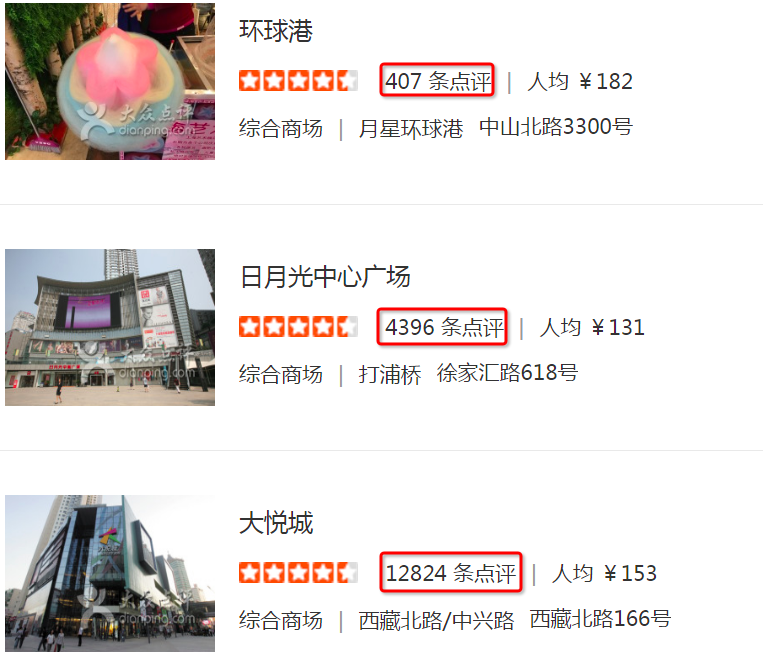
\includegraphics{figures/features/dianping.png}}
	\caption{POI listings of businesses on Dianping.com}
	\label{fig:dianpingexample}
\end{figure}


Then we spatially cluster only those popular POIs from each category
by affinity propagation (AP) algorithm \cite{frey07affinitypropagation}.
The advantage of AP is that we do not need to preset the number 
of clusters. We thus obtain a number of functional areas within 
the city, such as the those shown in \figref{fig:routing}. Here,
blue, purple and red dots represent cluster centers for
residential, shopping and business areas respectively.
Next we compute the fastest routes between any two cluster centers 
over the road network by an A* search algorithm~\cite{4082128}. 
The road network is first remodeled as a 
weighted undirected graph before the routing takes place. 
The weight on each edge is determined by the type of the road 
and its speed limit. An example route 
between two cluster centers is shown as a green line 
in \figref{fig:routing}.

\begin{figure}
	\centering
	\resizebox{\columnwidth}{!}{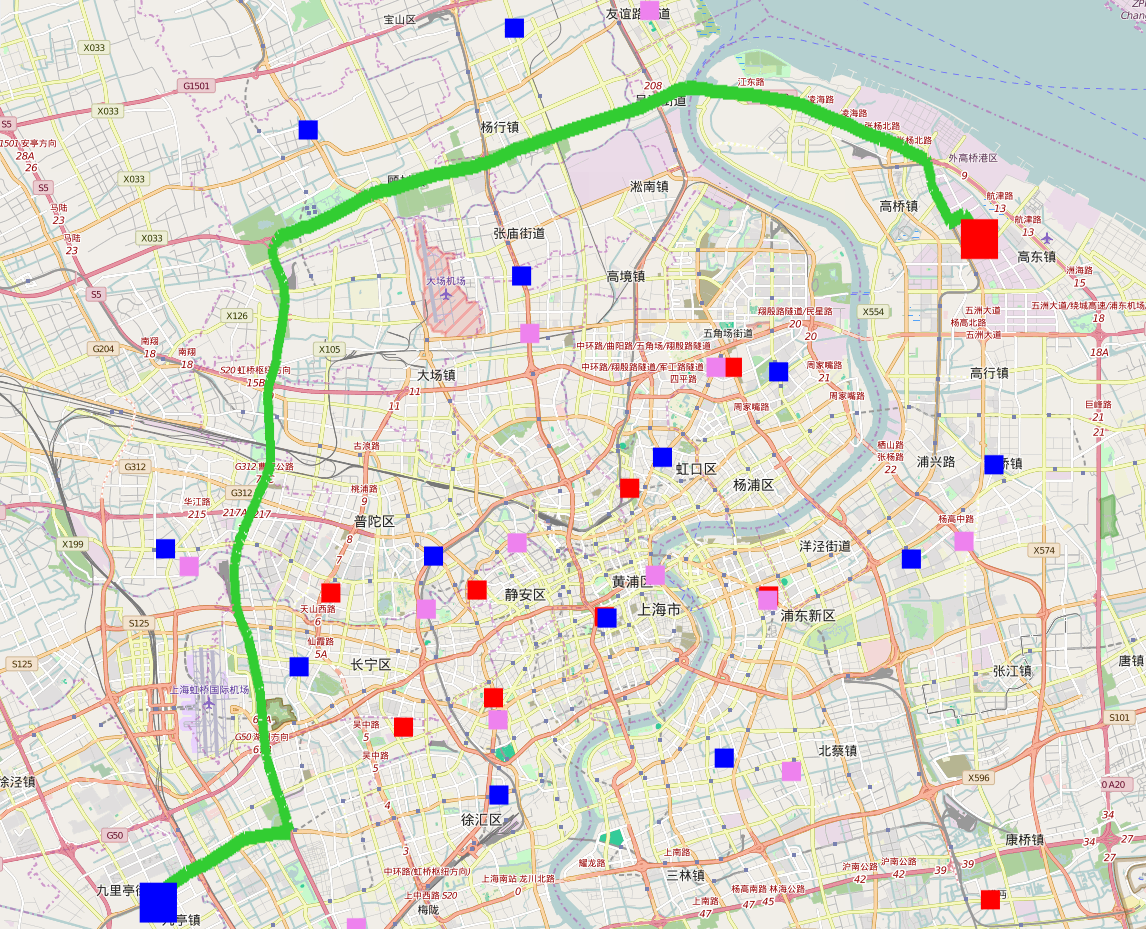
\includegraphics{figures/features/routing.png}}
	\caption{An example graphical output of the optimal routing program from one place to another}
	\label{fig:routing}
\end{figure}

Nine global features are then added to each road node on OSM to represent 
the number of times this node is on the fastest way between any two functional
areas~\footnote{There are $3\times3 = 9$ combinations of travel patterns.}.

%the hot or popular ways, which are the numbers of occurrences for this node to be in the all routes between those 3 clusters of functional areas. To be clear, there are the number of the best routes between residential areas and business site areas that passes just through this particular node, and the number between residential areas and shopping mall areas as well as the number between business sites area and shopping mall areas. In this way, we can have each node having the features that represent the level of popularity of itself as being chosen by people when thinking of driving from on cluster to another.


%As stated in the above section, the local features already play a large part of the roles in the features. However, not all traffic problems and behaviors are only related to the locality of the place where all the cars and traffic goes through. Actually we need to figure out a way to describe and better understand the driver’s motivation and habits. People do not just drive around the city finding the shops or the supermarkets on the sides of the road, they drive every day to work and back home. These commuters are making up a large portion the traffic jam that happens every day on rush hours like in the morning or in the late afternoon on elevated roads, highways, etc. Taking an example in Shanghai for example, many people lives in the suburban areas that is outside the outer ring road of the city. Most of the large companies that is really having large numbers of employees are most possibly located in the urban area inside the middle ring road. A long journey and distance for commuters is a great example showing that local geospatial data are not enough. It does not capture the potential information of where the people would most likely come from and where would they most likely. Temporal data also affecting the problem. In the weekdays, rush hours’ drivers contribute to the most of the traffic jam situations, on the other hand, in the weekend, many people would stay in some shopping mall and going out to the city center to have a nice dinner. The peak traveling hours are varying and changing.

%After proposing that local features are not sufficient, we need to figure out a quantitative set of features that best describe the driver’s preference on roads. Some roads will get really crowded and slow because too many drivers are going to choose the route including the road. For example, every morning and late afternoon, the S4 Hujing Expressway and Humin Elevated Road are both under heavy traffic because there are many people living in the Minhang District of Shanghai, which is a large place for residential areas. The road is also the easiest road to drive that connects the urban area of Xujiahui District, which has all the commercial buildings and shopping malls. Examples like this exists in all aspects of urban life and are quite common. Actually most people on the road lives in the similar place and go to work or eat in the similar places too, and because of the clustering property of human society and urban planning, that gives one of the reasons why roads are crowded. That is we need to identify the “functional areas” in the city that has three types of functionality: shopping, residential and commercial.

%In order to solve this, we need to first find out where people usually live, which is the residential area in the city; where people usually drive to work, which is the business area in the city; and where people usually dine outside and go shopping, which is the commercial area in the city. We need to find out those large clustered points of interest by using clustering algorithms.
%
%\paragraph{Obtaining Data for Clustering}
%Before trying out a variety of the clustering algorithms, we need to collect the raw data first and then apply those algorithms to them. Currently in our database, we have the OpenStreetMap’s geospatial data like road network maps, and the nodes (which we also call them points of interest) crawled, processed and loaded into the database. It seems that we already have solid knowledge base on the sheer number of POIs we have now. However, we lack the popularity of the points of interest information. We wanted to know how many people and how frequently people would go to the specific shopping mall or which building have large amounts of employees that work there. An approach is designed to solve this lack of knowledge problem by cross referencing and collaborate with crawled data of other websites. In our case, we used two external data source, Dianping.com and place.weibo.com, which is both very popular among Chinese people and have a large user base. We primarily used the Dianping.com for the extensive categorical points of interest information of the names, address, rating, price as well as the comments and number of comments of the point. We wrote a Python crawler script to crawl a whole set of data from Dianping.com, mainly consisting 3 types of the functional areas: shopping malls, residential areas and commerce buildings in Shanghai. See Figure~\ref{fig:dianpingexample} for an example page with information of the places. 
%
%After we obtained the places in Shanghai from Dianping.com, we can parse the information of each place obtained. A special program is written to parse the Chinese address shown in the webpage, and extracts only the road name and city name in it. It is actually an address parser using extensive regular expressions to match the address in format that could extract the name of road. The reason for this is to have a better link between the name and address, and better support fuzzy matching while later searching on Weibo Place. Normally there are many shops and restaurants in one shopping mall, and many companies in one business building, so with the help of address parsing, it is much more accurate to find all places associated to that large place. Place.weibo.com is a website for searching location based information that people attached with their status provided by Weibo, a popular social media network in China, that supports searching the place with keywords. Its result is useful for us to determine and quantize the popularity among the people of given place of interest that we obtained earlier in Dianping.com. As shown in Figure~\ref{fig:weiboexample} the information of the search result of a specific place contains the number of posts containing the location, and how many people have come here before and the number of photos users have uploaded.
%\begin{figure}
%	\centering
%	\resizebox{\columnwidth}{!}{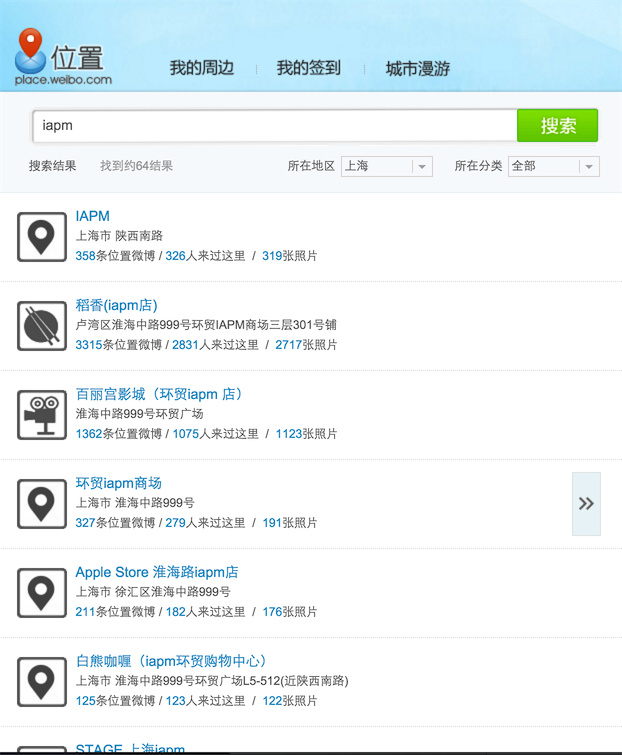
\includegraphics{figures/features/weibo.jpg}}
%	\caption{An example page of the location name search results of Weibo on place.weibo.com}
%	\label{fig:weiboexample}
%\end{figure}
%
%We search for each of the places in Weibo Place by place name that we obtained earlier in Dianping.com and filtered the search result with the road name parsed from the address to ensure that only places with the same address are being counted. The sum of those numbers of posts, photos, check-ins are saved to output file, which will be processed to be our data for clustering later. We sorted by the sum as popularity of the place inside the whole lists of those places, and get a top 1000 most popular list of places of business sites, residential areas and shopping malls. We have made the plots of these data as scattered data in geographical coordinates. See Figure~\ref{fig:businessareas},~\ref{fig:shoppingareas} and~\ref{fig:residencearea} for the distribution and density of each of the 3 functional areas. X-axis dimension is the latitude and Y-axis dimension is the longitude.
%\begin{figure}
%	\centering
%	\resizebox{\columnwidth}{!}{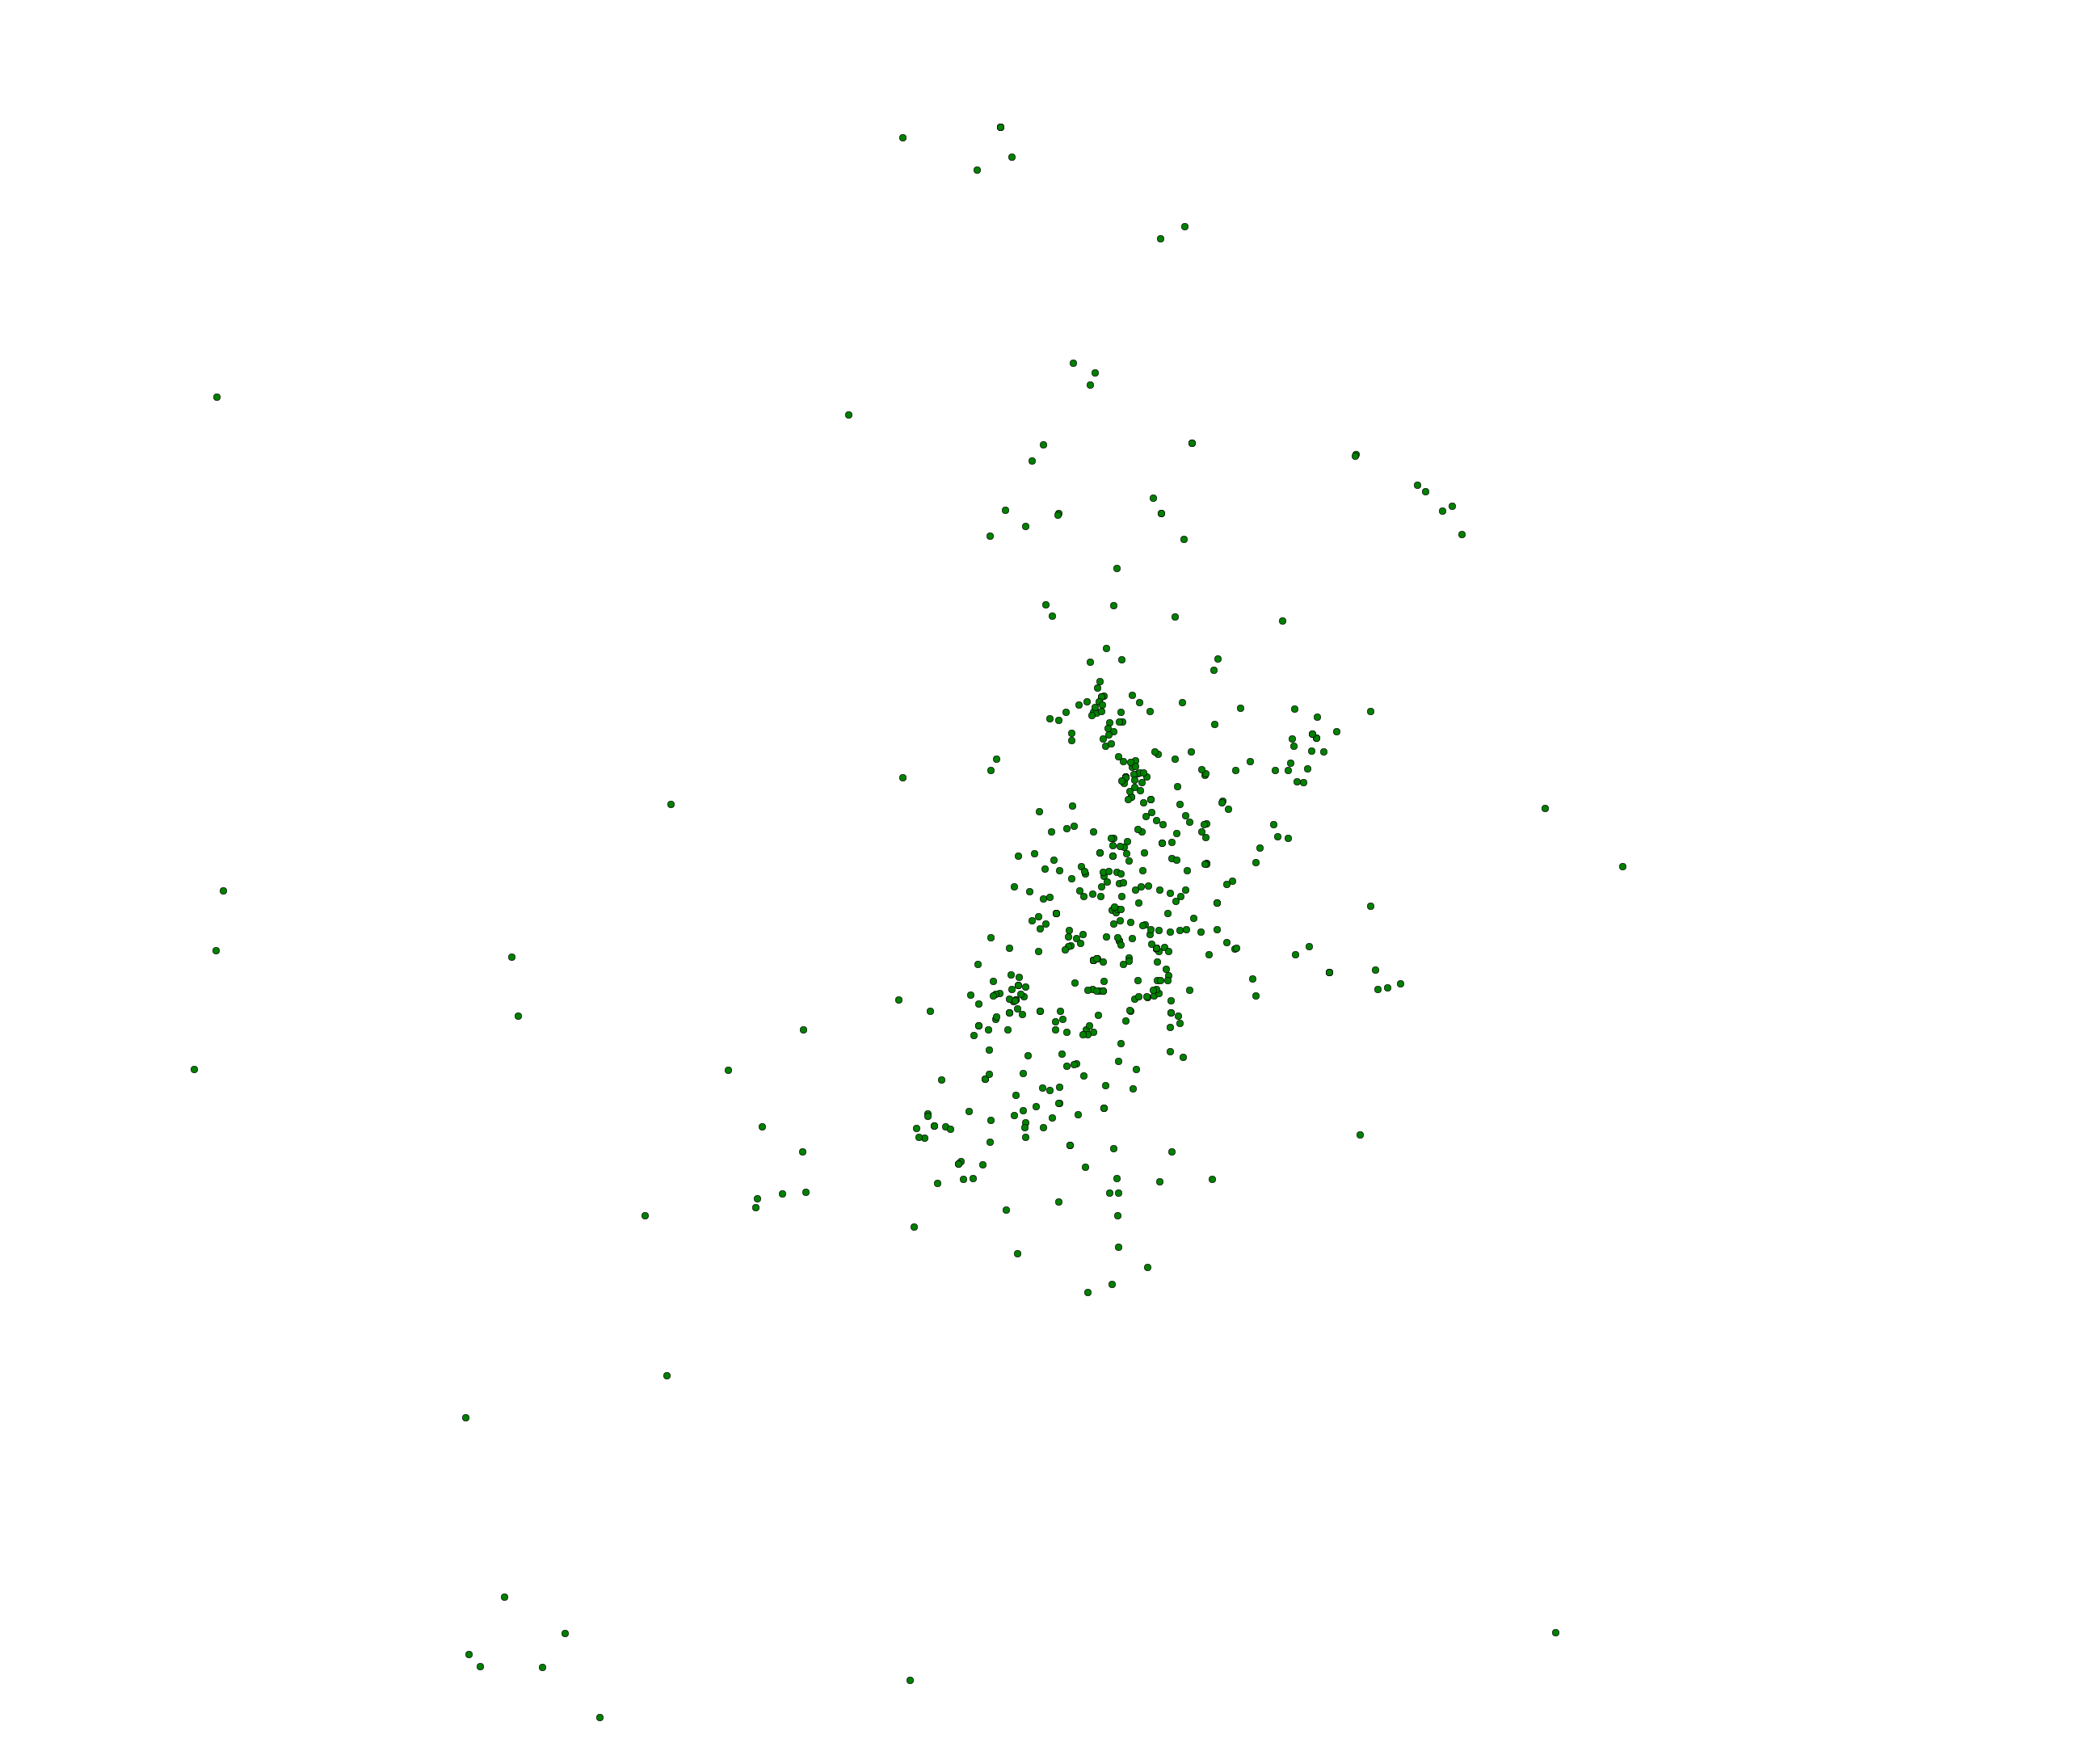
\includegraphics{figures/features/businessSite.png}}
%	\caption{Scattered plot of top business site areas in Shanghai}
%	\label{fig:businessareas}
%\end{figure}
%\begin{figure}
%	\centering
%	\resizebox{\columnwidth}{!}{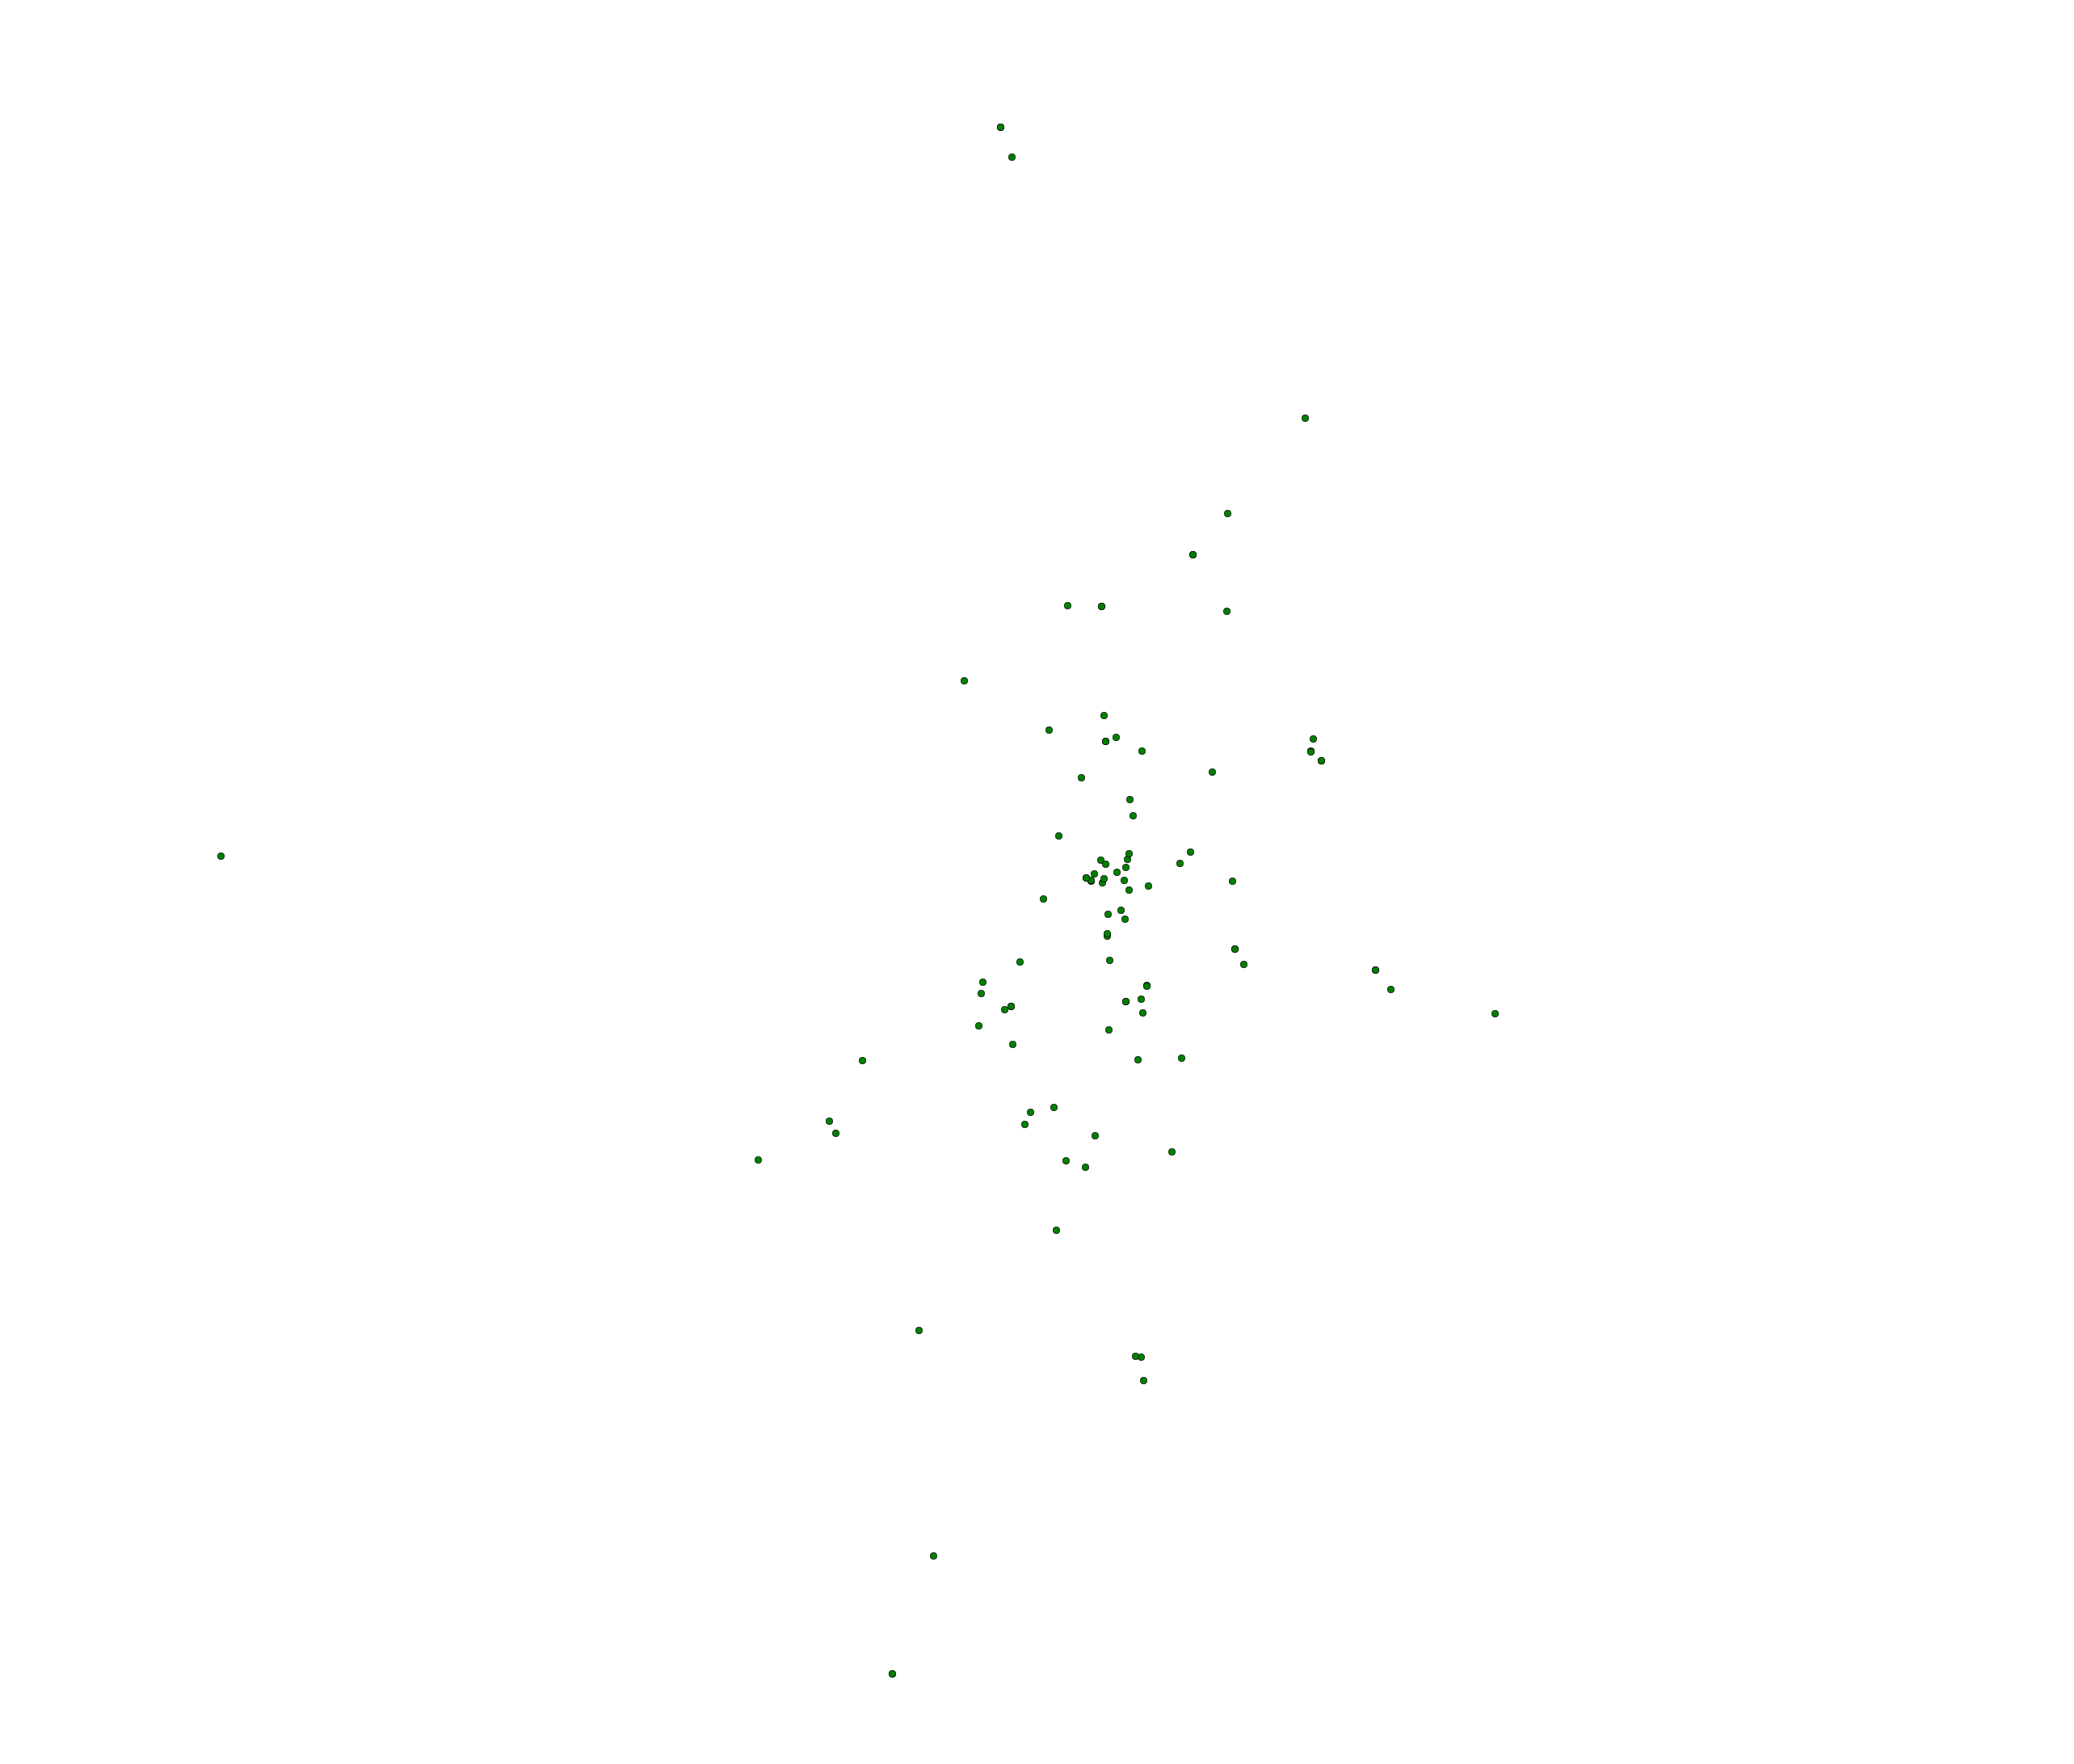
\includegraphics{figures/features/mall.png}}
%	\caption{Scattered plot of top shopping mall areas in Shanghai}
%	\label{fig:shoppingareas}
%\end{figure}
%\begin{figure}
%	\centering
%	\resizebox{\columnwidth}{!}{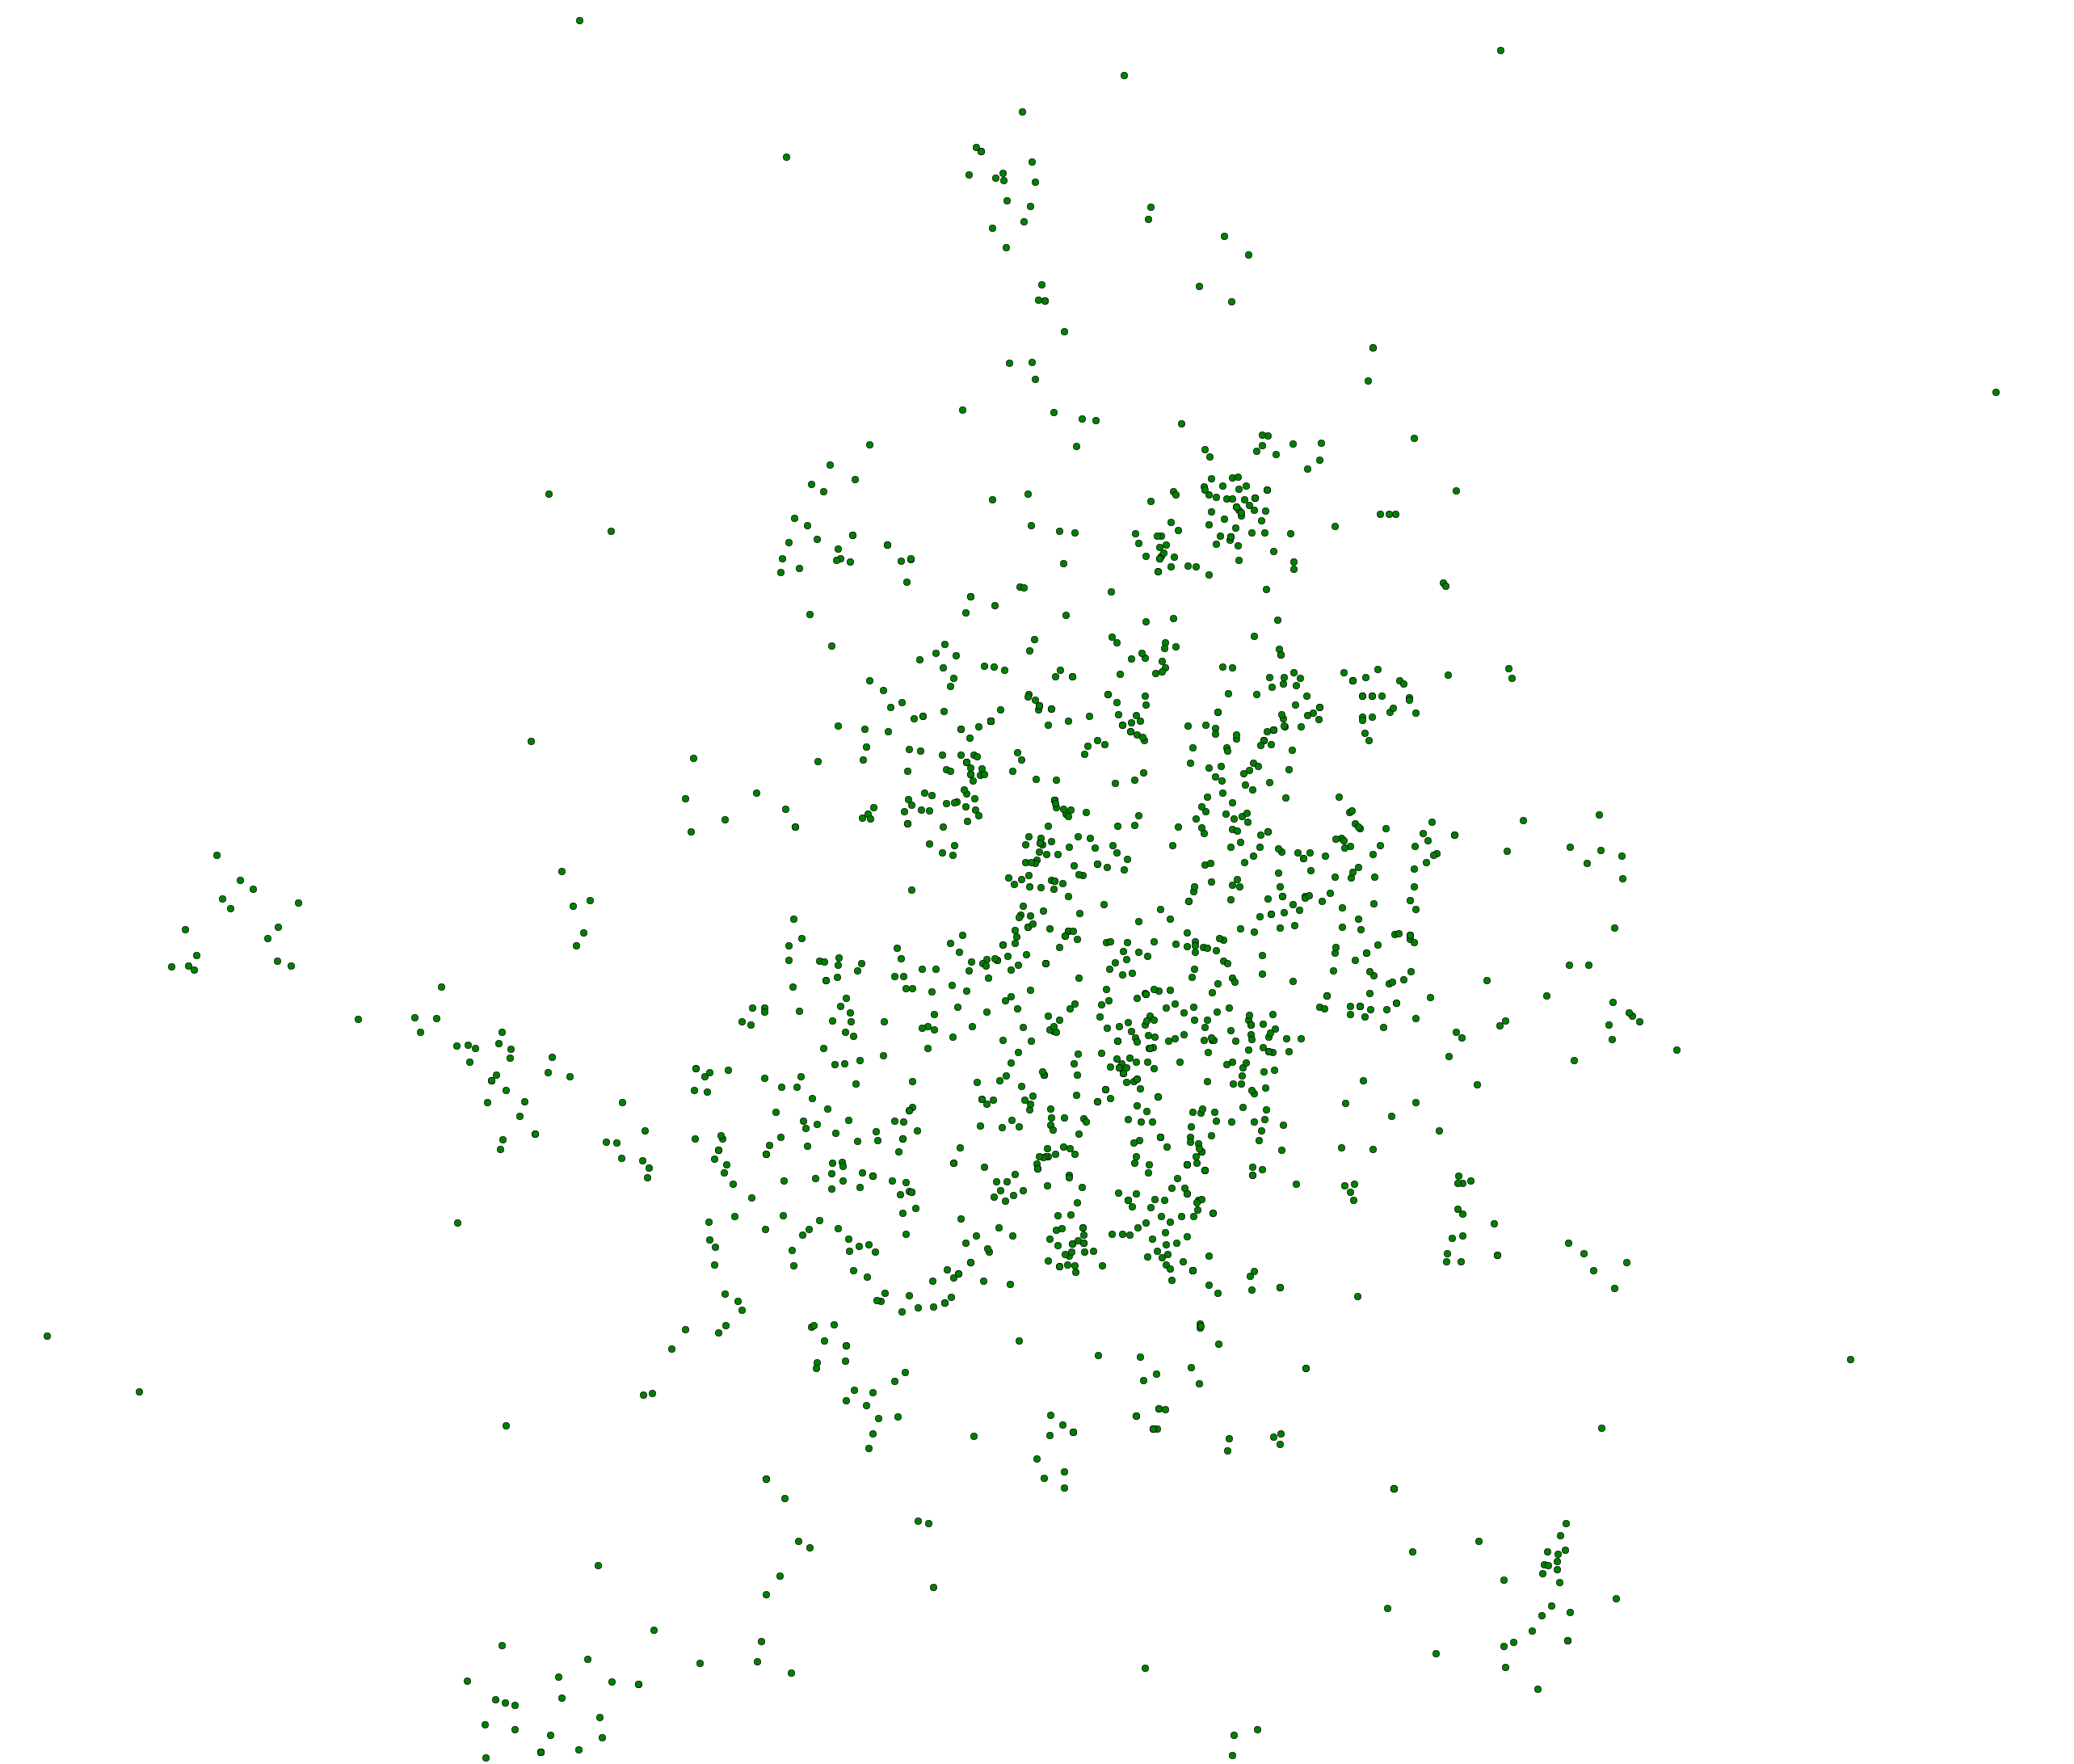
\includegraphics{figures/features/residence.png}}
%	\caption{Scattered plot of top residential areas in Shanghai}
%	\label{fig:residencearea}
%\end{figure}
%
%\paragraph{Clustering the Data Collected}
%Now that we have processed top 1000 most popular lists of three types of places, we can apply the clustering algorithm to find out the clustered functional areas that we wanted. Several of the famous and popular clustering algorithms exist, but the methods of clustering mainly fall into two categories: the first is hierarchical (agglomerative) that initially, each point is in cluster by itself, and then repeatedly combine the two “nearest” into one. The second is point assignment, that is it maintains a set of clusters, and place points into their “nearest” cluster. Many algorithms exist for dealing with such problems, for example the very famous algorithm called the k-means, as well its variant BFR (Bradley-Fayyad-Reina) algorithms for large dataset and some other hierarchical clustering methods, DBSCAN, and Gaussian Mixtures, etc. In this case, however, after studying and experimenting with those algorithms, we selected to use Affinity Propagation algorithm \cite{frey07affinitypropagation}. It's said to be fast, efficient and do not need to specify the number of cluster beforehand, which suits our case well since we want fully automatic clustering without knowing how many those different functional areas there are. It creates clusters by sending messages between pairs of samples until convergence. A dataset is then described using a small number of exemplars, which are identified as those most representative of other samples. The messages sent between pairs represent the suitability for one sample to be the exemplar of the other, which is updated in response to the values from other pairs. This updating happens iteratively until convergence, at which point the final exemplars are chosen, and hence the final clustering is given. Affinity Propagation can be interesting as it chooses the number of clusters based on the data provided. For this purpose, the two important parameters are the preference, which controls how many exemplars are used, and the damping factor.
%The main drawback of Affinity Propagation is its complexity. The algorithm has a time complexity of the order $O(N^2 T)$, where $N$ is the number of samples and $T$ is the number of iterations until convergence. Further, the memory complexity is of the order $O(N^2)$ if a dense similarity matrix is used, but reducible if a sparse similarity matrix is used. This makes Affinity Propagation most appropriate for small to medium sized datasets. 
%
%Algorithm description: The messages sent between points belong to one of two categories. The first is the responsibility $r(i, k)$, which is the accumulated evidence that sample $k$ should be the exemplar for sample $i$. The second is the availability $a(i, k)$ which is the accumulated evidence that sample $ i $ should choose sample $ k $ to be its exemplar, and considers the values for all other samples that $ k $ should be an exemplar. In this way, exemplars are chosen by samples if they are (1) similar enough to many samples and (2) chosen by many samples to be representative of themselves.
%More formally, the responsibility of a sample k to be the exemplar of sample i is given by:
%\begin{align}
%r(i, k) \leftarrow s(i, k) - max [ a(i, \acute{k}) + s(i, \acute{k}) \forall \acute{k} \neq k ]
%\end{align}
%Where $ s(i, k) $ is the similarity between samples i and k. The availability of sample k to be the exemplar of sample i is given by:
%\begin{align}
%a(i, k) \leftarrow min [0, r(k, k) + \sum_{\acute{i}~s.t.~\acute{i} \notin \{i, k\}}{r(\acute{i}, k)}]
%\end{align}
%To begin with, all values for $ r $ and $ a $ are set to zero, and the calculation of each iterates until convergence.
%
%We used the open source machine learning library called scikit-learn \cite{pedregosa2011scikit} which has the affinity propagation algorithm included. So we simply feed the data in with a small Python script and we have some quite amazing clustering result. For example, in the clustering of the data of top business sites obtained earlier, eventually it generates 23 clusters and the Silhouette Coefficient is 0.63. It means that it works relatively good. If the ground truth labels are not known, evaluation must be performed using the model itself. The Silhouette Coefficient is an example of such an evaluation, where a higher Silhouette Coefficient score relates to a model with better defined clusters. The Silhouette Coefficient is defined for each sample and is composed of two scores:
%a: The mean distance between a sample and all other points in the same class.
%b: The mean distance between a sample and all other points in the next nearest cluster.
%The Silhouette Coefficient s for a single sample is then given as:
%\begin{align}
%s = \frac{b - a}{max(a, b)}
%\end{align}
%The Silhouette Coefficient for a set of samples is given as the mean of the Silhouette Coefficient for each sample. The score is bounded between -1 for incorrect clustering and +1 for highly dense clustering. Scores around zero indicate overlapping clusters. The score is higher when clusters are dense and well separated, which relates to a standard concept of a cluster. For clustering result, we can see Figure~\ref{fig:clusteroutput} for the clustered output’s plot of the top business sites found. Those clusters are exactly the functional areas of this particular type that we discussed earlier and at first glance it seems good.
%
%\paragraph{Routing between Functional Areas}
%In the previous chapter, we used the affinity propagation algorithm to cluster the top popular points of interest for each type of the three category. At the time we have three sets of the functional areas of the type business site, residential area and shopping area. We have the knowledge of where they are located at, since the cluster algorithm returns an exemplar for representing the whole nearby area. In order to reflect this information on the road network, we need to find out the connecting routes that people and commuters use for going to work and back home as well as to malls for eating and shopping. Imagine a scenario that a person who lives in Minhang District near Shanghai Jiao Tong University, is working in a company located at Xujiahui. So his living area is actually within the functional area of residence, and Xujiahui is both a business site area and shopping mall area. For his weekdays, he would most probably take the S4 Expressway and into Humin Elevated Road to get to work, so these highways will be under heavy traffic during rush hours, making all the nodes and way segments on it a popular way of choice On Friday night after work for example, he would like to drive to the South Shanxi Road to have dinner in IAPM shopping mall and shop there with his girlfriend, so on such a weekend night, he would take Huaihai Road to move from the business site area to a shopping mall area, and Huaihai Road may become very crowded for this popularity, and so does the nodes on this road. 
%
%In order to find out what ways are popular or not because of the reason that these nodes and segment on this particular way are the connecting components that lies on the road among which is crucial in the most popular routing choice. As many people would use navigation software, finding the recommended routes between those discovered types of functional areas now proves to be important.
%
%When talking about routing algorithms on a road network, we would instantly consider the map information being represented as a directional graph with weight on the edges. The edges would be the road segments connecting nodes. Our new problem of finding the most popular route between two locations now is being translated into the problem of finding the shortest path in a large graph between two vertices. To be more accurate, it should be the cheapest cost path because we do not just want the route that is short in mere distance, we would like to take road type and so on into consideration. So a weighted shortest path problem should best describe this, and the weight is affected by road type, for example the elevated roads or highway that have a better speed and priority should cost less weight than the secondary and ordinary roads with crossings and traffic lights making them more favorable. Also, one-way is also an important deciding factor in routing algorithms because it would simply disable or prohibit such edges being reached in certain direction. In our database there is always a tag with the way elements, showing the road hierarchy and one-way flag.
%
%We consider a directed graph $ G = (V,E) $ with n nodes and $ m = Θ(n) $ edges. An edge $ (u,v) $ has the non-negative edge weight $ w(u,v) $. A shortest-path query between a source node $ s $ and a target node $ t $ asks for the minimal weight $ d(s, t) $ of any path from $ s $ to $ t $. In static routing, the edge weights do not change so that it makes sense to perform some pre-computations, store their results, and use this information to accelerate the queries. Obviously, there is trade-off between query time, pre-processing time, and space for pre-processed information. In particular, for large road networks it would be prohibitive to pre-compute and store shortest paths between all pairs of nodes.
%
%Dijkstra’s Algorithm \cite{dijkstra1959note} is the classical algorithm for route planning—maintains an array of tentative distances $ D[u] ≥ d(s, u) $ for each node. The algorithm visits (or settles) the nodes of the road network in the order of their distance to the source node and maintains the invariant that $ D[u] = d(s, u) $ for visited nodes. We call the rank of node $ u $ in this order its Dijkstra rank $ rks(u) $. When a node u is visited, its outgoing edges $ (u,v) $ are relaxed, i.e., $ D[v] $ is set to $ min(D[v], d(s, u) + w(u,v)) $. Dijkstra’s algorithm terminates when the target node is visited. The size of the search space is $ O(n) $ and $ n/2 (nodes) $ on the average. We will assess the quality of route planning algorithms by looking at their speedup compared to Dijkstra’s algorithm, i.e., how many times faster they can compute shortest-path distances.
%
%The algorithm that we use in our routing purpose is A* Search algorithm \cite{4082128}, also known as Geometric Goal Directed Search. The intuition behind goal directed search is that shortest paths ‘should’ lead in the general direction of the target. A* search achieves this by modifying the weight of edge $ (u,v) $ to $ w(u,v)−π(u) + π(v) $ where $ π(v) $ is a lower bound on $ d(v,t) $. Note that this manipulation shortens edges that lead towards the target. Since the added and subtracted vertex potentials$  π(v) $ cancel along any path, this modification of edge weights preserves the shortest paths. Moreover, as long as all edge weights remain non-negative, Dijkstra’s algorithm can still be used. The classical way to use A* for route planning in road maps estimates $ d(v,t) $ based on the Euclidean distance between $ v $ and $ t $ and the average speed of the fastest road anywhere in the network. Since this is a very conservative estimation, the speedup for finding the quickest routes is rather small. Lastly there is heuristic that evolved during recent years. In the last decades, commercial navigation systems were developed which had to handle ever more detailed descriptions of road networks on rather low-powered processors. Vendors resolved to heuristics still used today that do not give any performance guarantees: use A∗ search with estimates on $ d(u,t) $ rather than lower bounds; do not look at ‘unimportant’ streets, unless you are close to the source or target. The latter heuristic needs careful hand tuning of road classifications to produce reasonable results but yields considerable speedups.
%
%In the engineering process, we implemented A* algorithm to read the OpenStreetMap data format, along with two coordinates representing the starting point and ending point of the routing. We used the tags about the road that the ways in the database have to create a customized weight for different type of roads. We are routing each location in the clustered functional areas to those other locations in another type of functional areas. So we have 3 groups of routing being done: the routes between locations in residential areas and business sites areas, the routes between locations in residential areas and shopping mall areas, and the routes between locations in business sites areas and shopping mall areas. An example routing after running our program is plotted in Figure~\ref{fig:routing}, note that the map plots all valid roads of the bounded area in Shanghai, and the red polylines which take a large majority is the roads that has not been searched. Those in blue are the roads that the A* algorithms runs through and calculated. The green one is the final optimal route found. We have all the node ID and way ID information so that we can identify easily.
%

\subsubsection{Non-Geospatial Implicit Features}

The following features are not properties of the map, but may have implicit impact
on the population density of an area, the drivers behaviros, or the travel patterns.
We proposed 8 features in this category: 
\begin{itemize}
\item the time of the day (in hours); 
\item weekday or weekend; 
\item the 1-, 2- and 3-bedroom apartment rental price in the area; 
\item the temperature in the day and night; and 
\item the weather condition of the time (i.e., sunny, cloudy, shower or rainy, etc.). 
\end{itemize}
%It is quite straightforward for us to come up with these features, they can have linkage with the traffic situation. For example, the rental price of the nearby apartment reflects the popularity, population and land price of the area, which shall further imply the degree of importance and centrality in urban area. There are really some expensive residential areas in Shanghai like near the center of the city in Huangpu District, where the population is really high. The population density is a crucial matter that affects traffic. If the rental price is high, it means that there lives a high density of people, and as a result, the traffic vehicles that travels from and to this place will be massive, resulting in heavy traffic. So we think it is a significant feature that represents the population density of the area, the distribution over area data of which is hard for us to obtain. 

%Other features like the time of the day and the difference between weekdays and weekends are also self-explanatory: people have different goals and motivation of where they would like to drive to on weekdays and weekends, which will affect road network loads and as a result causing traffic problems. In rush hour of weekdays, the roads' connection where most people live and where the workplaces being located at are getting large flow of traffic. On weekends however, roads connecting the residential functional areas and shopping mall areas during the dinning time and the closing hour of the shopping mall will also become under heavy congestion. Other features like weather and temperature of the area are also straightforward and guaranteed to have positive effects on prediction results. When the weather is rainy and bad, by all our consensus, people tend to drive more than walking and taking public transit because of the bad weather makes people reluctant to spend time outside and rather to stay inside the cars. Also the speed of vehicle under bad weathers are lower than normal, contributing to the congestion. Extremely low and high temperatures will also cause the people drive more often because there is air conditioning inside and without the hassle and of walking outside.

%In summary, here we list all the features we discussed in this
%section. 
%%
%%
%%
%\begin{itemize}\itemsep0pt
%	\item local geo-spatial
%	\begin{itemize}\itemsep0pt			
%		\item POI
%		\item road density
%		\item road type
%		\item haveshop 
%	\end{itemize}
%	
%	\item global geo-spatial
%	\begin{itemize}\itemsep0pt			
%		\item routing
%	\end{itemize}
%	\item non-geo-spatial
%	\begin{itemize}\itemsep0pt			
%		\item price
%		\item temperature
%		\item weather
%		\item hour
%		\item isweekend
%		\item isRushHour
%	\end{itemize}
%\end{itemize}

%with a total number of 311. Note that the weather condition feature is represented as a binary representation of 1-in-N representation, see Section~\ref{sec:modelextractfeature} for details. Some of those features are input by user as prior knowledge during the prediction step. Though with different source and magnitude, either explicitly or implicitly representing the causing factors, they, being put together, comprise a large set of knowledge engineered by either we researchers as well as the computer algorithms, and that is one of the most important step and effort in application machine learning in real world scenarios.

% DO WE NEED TO ADD FEATURE LIST HERE?


